\section{Motivation}
\label{motivation}

\begin{figure}[b]
	\centering
	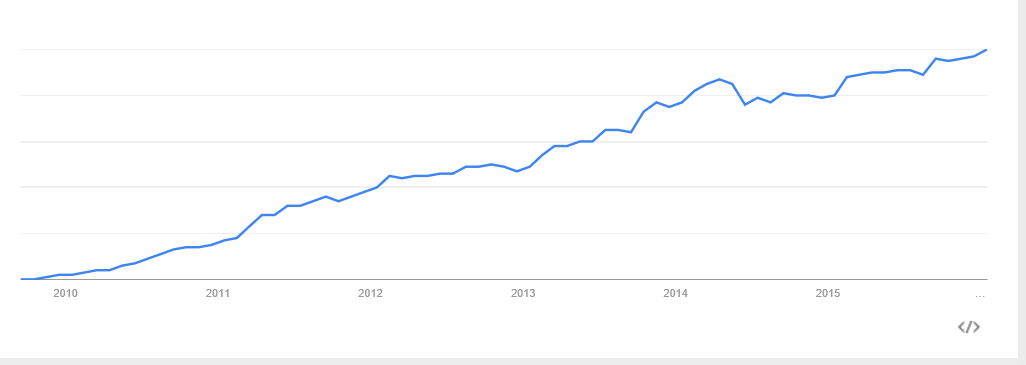
\includegraphics[width=0.7\linewidth]{figures/NodeJS.png}
	\caption{Steigerung der Suchanfragen für NodeJS. Datenquelle: Google Trends \cite{googleTrends:nodeJS}}
	\label{f:motivation:nodejs}
\end{figure}

Ein Großteil aller Webanwendungen ist in der Skriptsprache PHP geschrieben. 
So werden über 81\% aller Anwendungen damit geschrieben und ein demgegenüber verschwindend geringer Anteil von nur 0,1\% in JavaScript \cite{w3techs:serversidePLUsage}.
Es ist jedoch ein klarer Trend zu JavaScript als Programmiersprache erkennbar, weshalb es sinnvoll ist sich näher mit dem MEAN Stack zu befassen.
Das Interesse ist in den letzten Jahren linear gestiegen.
Dies wird auch aus der Abbildung \ref{f:motivation:nodejs} ersichtlich.
Dort ist die Steigerung an Suchanfragen zu dem Thema NodeJS angegeben.
Google Trends liefert zwar keine absoluten Zahlen der Suchanfragen, jedoch lässt sich erkennen, dass die Anfragen sich in den letzten 5 Jahren stetig steigern konnten. 
Auch ist der Bekanntheitsgrad der anderen drei Komponenten stark gestiegen.
Selbst große Firmen wie Uber\cite{buildwith:uber.com}, Red Bull\cite{redbull:job} oder Netflix\cite{infoq:netflix} setzen Teile davon ein.
Oftmals wird dies durch eine verkürzte Entwicklungszeit zur Erstellung von Webanwendungen und durch eine gesteigerte Performanz begründet.

Zudem hat es gewisse Vorteile für Unternehmen. So erleichtert es die Einführung von agilen Methoden.
Meist werden Aufgaben in die Teile Frontend und Backend aufgeteilt und von unterschiedlichen Personen erarbeitet:
Frontendentwicklern, die sich typichscherweise sehr gut mit den Technologien HTML, CSS und JavaScript auskennen und Backendentwicklern, die nur mit den serverseitigen Komponenten wie beispielsweise PHP und MySQL arbeiten.
Da im MEAN Stack, NodeJS, Express und AngularJS auf JavaScript basieren und sogar MongoDB JavaScript ausführen kann, können nun die Aufgaben anderes aufgeteilt werden.
So ist es nicht mehr nötig nach Frondend und Backend zu trennen sondern die Aufgaben vertikal zu schneiden, wodurch jeder Entwickler alle Bereiche eines Features bearbeiten kann.
Dieses Vorgehen wird unter anderem durch das Elephant-Carpaccio beschrieben \cite{cockburn:elephant}. 
Grund genug sich näher mit den einzelnen Komponenten zu befassen.